%Mega Man X
\chapter{X}\label{char:X}
\begin{figure}[h]
	\centering
	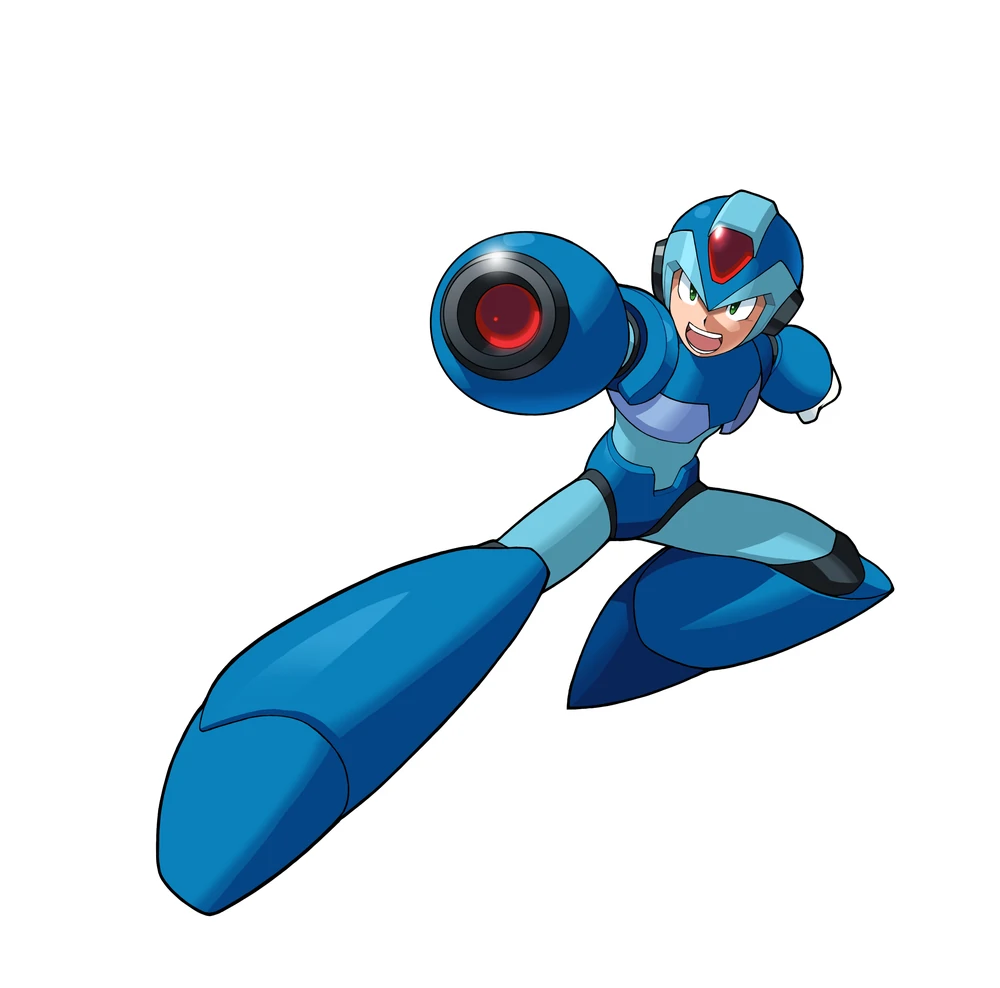
\includegraphics[width=0.6\linewidth]{figures/Characters/Char_MMX.png}
\end{figure}

X is the main protagonist of the Mega Man series which bears his name. He is the last creation of the brilliant Dr.~Light, a robot built with the gift of free will and limitless potential and a Maverick Hunter, appointed to stop reploids gone maverick to hurt human people. 
X's primary characteristic is his kind heart and peaceful attitude, which makes him repel violence, often trying to reason with his enemies. However, despite this attitude, X knows well the threat mavericks are and, even if unwilling, fight against them with all his strength to bring the world at peace.

\section{Technical Specifications}
X's specification can be found both in the opening scene of the first Mega Man X game and in the \emph{Rockman \& Rockman X Daizukan}~\cite{book:RRXD}-\cite{X_specs_translated} book. While some information overlap between these sources, others are exclusive to a single one, hence here both of them are reported as sources of information.

\paragraph{General Information}
\begin{itemize}
	\item Height: 160 cm.
	\item Weight: 57 Kg (lighter than Rock due technological improvements).
	\item Main energy source is Solar energy.
	\item Armor is composed of a lightweight ``Titanium-X'' alloy, the strongest metal in the world. Very light and resistant to heat and shots.
	\item Internal skeleton is a super elastic armor that can reduce received damage by approximately 93\%.
	\item A.I. age between 14 and 15 years old in human terms at the beginning of the first game. Matures as time passes.
\end{itemize}

\paragraph{Head equipment}
\begin{itemize}
	\item Eyes are constituted by broad-range cameras, giving him the ability to see more things the human eye can.
	\item Ears are composed of an ultra-high sound recognition system, allowing him to hear even ultrasonic sounds.
	\item Voice is produced by a voice generation system made by HAYATOM Inc. (MOKUOO Inc. in Japanese version). 
\end{itemize}

\paragraph{Chest equipment}
\begin{itemize}
	\item An Accumulative Energy Generation Device allows to accumulate solar energy and provide X with the sufficient amount of power required to work.
	\item A Micro-fusion fuel tank, which stores fuel for X to use when solar energy is not available, such as caves or underwater.
	\item A Central Joint-controlling system, which acts as X's secondary brain and controls his movements.
\end{itemize}

\paragraph{Leg equipment}
\begin{itemize}
	\item Gyroscopic Stabilization System/Full auto-balancer to help X in remaining stabilized and land properly from any state he's in.
	\item The Emergency Acceleration System, which enables X to accelerate at high speed in a short amount of time. This equipment is optional and must be installed in a second moment.
\end{itemize}

\paragraph{Arm equipment}
\begin{itemize}
	\item Mega Buster Mk.17 (X-Buster). X’s basic weapon built into his hand. When fighting his hand retracts and leave the place to the buster~\cite{elysium_weapons}
	\item Energy Amplifier to store and concentrate energy into a more powerful shot, the Charged Shot.
	\item Variable Weapon system: Allow the X-buster to transform and emulate attacks from enemies bosses. How the copy/learning process is performed remains, however, unknown.
\end{itemize}


\section{Creation}
X's creation begins in the year 20XX by the hand of famous scientist Dr.~Thomas Light. Reasons that brought Dr.~Light are to be found into two main facts that happened during the scientist's life. The first one was the coming of an unknown computer virus from space that caused robots to go violent (which could be a reference both to the ``Evil energy'' appeared in \emph{Mega Man 8} or the \textit{Roboenza} Virus appeared in \emph{Mega Man 10}). After this event Dr.~Light decides that a new battle robot had to be created in order to protect the future of earth~\cite{mega_man_network:Zero_timeline}, and starts building X. On why creating X and not upgrading Rock, the original \textit{Mega Man}, many hypothesis can be formulated, one being the fact that Rock was originally designed to help with laboratory work and not to fight, hence the preference to create a new robot, instead altering Rock too much. In addition, since the new robot to be created may fight other robots infected with viruses, a new anti-virus system had to be created within him. This last statement fits perfectly with the second reason Dr.~Light began creating X, which is his dream to create a robot who could choose his own path in life, effectively having free will. How it is possible to see from his journal~\cite{Dr.Light_journal}, in fact, the idea of a free-will was born and stayed in him from shortly after events of the first \textit{Mega Man} game up until X's creation, as he believed it was his duty to accomplish such achievement\footnote{\textit{If a robot posses the intelligence to be conscious of the possibility of opposing a human for the right reasons, will it be possible for them to worry aver what path is right? [...] I can sincerely feel that coming to think of this is my duty.} Dr.~Light's journal, 29 March 2017}. Furthermore as Roll pointed to Light, free will also create the perfect anti-virus system, as would made impossible for a robot to be manipulated\footnote{\textit{``If artificial intelligence can be aware of its own intelligence, then one can fix any kind of tampering'' [...] However if that very kind of electronic intelligence can realize ideas like hers} (Roll) \textit{, then I think it's possible to establish a consciousness that cannot be manipulated} Dr.~Light's journal, 7 March 2017}. 
\begin{figure}[htp]
	\centering
	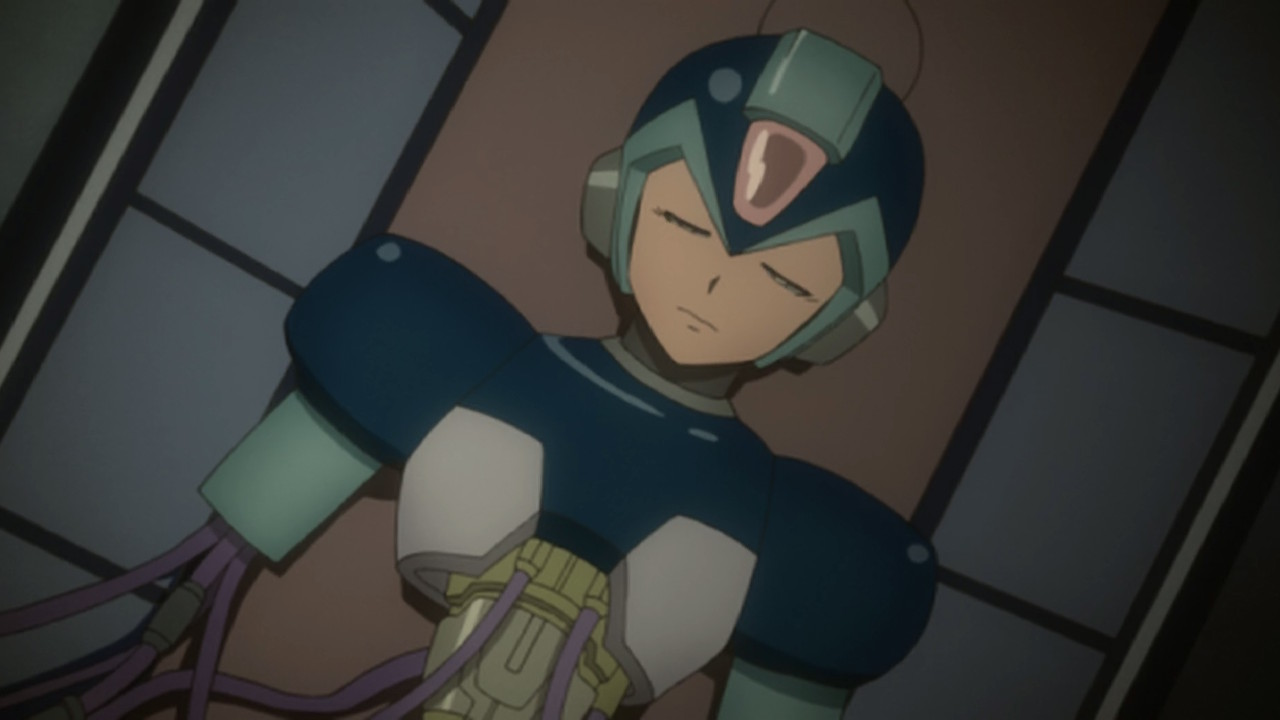
\includegraphics[width=0.7\linewidth]{figures/Characters/Char_X_build.jpg}
\end{figure}
It is unknown how long it took for Dr.~Light to complete X but, observing from the \emph{Day of $\Sigma$} OVA, it is possible to imagine that the development took most of Light's remaining lifetime as flashbacks show a doctor growing older and weaker as time passes.  During this time period however Light realizes the importance of his project and its impact it could have on the world due the power X holds, making him also realize the danger X could represent\footnote{\textit{``The name "X" also carries connotations of danger''}.} if, should the world turns against him, he takes a wrong path in life or begins to question the first law of robotics, risking disasters even worse than ones created in Wily's incidents~\cite{elysium_light_warning}. To avoid this situation, while still believing in X's good heart (as seen in X's flashback in \emph{Day of $\Sigma$}), Dr.~Light decides that X's moral integrity has to be tested deeply before letting him free. According to his studies, Dr.~Light estimates that about thirty years of testing should be necessary to completely ensure X's safety, time far beyond his own lifespan. For this reason, being near the end of his life and not having anyone who could continue his work, Dr.~Light creates a special capsule for X to rest in, capable of performing tests without the need of someone supervising it while also ensuring X's safety. After giving X farewell, on date 19$^{th}$ September 20XX, Dr.~Light proceeds to seal him away and leaves a message (written or recorded depending on the game) for whoever will find the capsule, explaining who X is and why he's special.

\section{Awakening and birth of reploids}
X's sleep last for about hundred years inside Dr.~Light's laboratory, buried underground and hidden from everything. It is only in 21XX the Dr.~Cain, a scientist of that time, while searching for plant fossils  from Mesozoic (or preserved plant from Middle Age~\cite{elysium_Cain_journal} in the Japanese version) accidentally finds the hidden laboratory. After some digging, Dr.~Cain manages to get in, where he first finds Light's note and documentation relative to X and, the following day, X's capsule itself still working. After reading Light's last note and warning message and checking the capsule status, which as stated in the journal show all indicators on green, on the 14$^{th}$ April 21XX Dr.~Cain awakes X from his slumber. Immediately after meeting him, Cain realizes how incredible and futuristic Light's creation is, even to his times, and decides to bring him, along all Light's design notes, to his laboratory in order to try to replicate X's design and create a similar robot.

More than six months were needed to complete the first robot, but on the 22$^{nd}$ November Dr.~Cain manages to create a robot using Light's schematics and X as reference. This new robot, just like X, is fully capable of making decisions on his own, even arriving to argue with Cain himself, to his surprise. However the new robot created isn't a perfect copy, as part of X's design couldn't be analyze even with modern technologies forcing Dr.~Cain to fix missing elements at his best, especially components constituting his ``\emph{Distress Circuit}''\cite{book:RMZ_Complete_works} which allows X to choose his side in society, and the new robot's moral integrity wasn't tested deeply as X's one. However since these differences seem to cause no problems, Dr.~Cain decided to start mass production of this new kind of revolutionary robot, which he named ``\emph{Reploids}''  (or \emph{Repliroids}).

It took not so long for reploids to integrate inside the society as Dr.~Cain himself notes in his diary in an entry dated 3$^{rd}$ May, where he states that \textit{everyone seems to be happy to accept them}. Reploids in fact began to work in place of and together with humans in all kinds of jobs, especially more dangerous ones which could put humans life at risk. However the situation won't last long,  as first mavericks will shortly start to appear.

\section{Mavericks and Maverick Hunters}

In the following entry in Cain's journal dated 16 July the scientist states: ``\textit{Three reploids went "maverick" today and injured two people before they were stopped. This is the third instance of this type of behavior and I still have no idea of what is causing it!}''. This entry describes the first mavericks occurrence in the series although, at the time the entry is written, they look more like isolated events related to some sort of explainable fault. However due the problem mavericks had caused, even with such a small number of occurrences (only three), the journal describes how the idea of halting the production already began to spread, but considering how society now depends on reploids, this idea is discarded from becoming reality. Instead a special organization called ``Hunters'' is  established in order to track down and halt mavericks before they cause any damage. Appointed leader of the organization is Sigma, Cain's latest and finest work equipped with last-design circuit which should prevent him from any fault Sigma also serves as leader of the 17th elite unit, operating on front lines against the maverick threat. X will join the organization only later in time (see \PtIIWarning), where will be assigned to the 17th unit under Sigma and where he will meet his future partner, Zero. 

Thanks to hunters' effort any further injure occurred as consequence of maverick attack, creating a situation of peace that lasted  for almost two years (two month in the English, see \PtIIWarning) During this period X fights together with his commander Sigma, his partner Zero and all his companions against mavericks, but deep inside he keeps questioning about his place in life and the path he has to choose\footnote{``\textit{I am a little worried about X. He seems unsure of his place in life and what Dr. Light had planned for him}'' Journal of Dr.~Cain, 10$^{th}$ December 21XX}.

\section{The X saga and the Maverick Wars}
On 4$^{th}$ July 21XX, Dr.~Cain 's worst nightmare becomes true. On this day Sigma goes maverick and begins his revolution against humanity, which he now considers an obstacle to Reploids' evolution that has to be eliminated. Together with him sides most of his subordinates Maverick Hunters longing to follow their leader as well as other reploids seduced by Sigma's charisma and strength. According to events shown in the \textit{Day of $\Sigma$}, Sigma's war declaration coincides with him storming a missile base and using it to attack Abel City, where the Maverick Hunter's headquarters reside. On this occasion X, together with Zero, have a first confrontation with him but both of them are defeated and injured. Before fainting, however, X manages to unleash a final attack on Sigma using all his strength, burning Sigma's scars in. After this last attack X shuts down, having used all his remaining power in the last hit, but Sigma decides to leave him there and to not deal the finishing blow, as Sigma now wishes X to reach his maximum potential and challenge him again, in order to discover the true power reploids hold.
\begin{figure}[htp]
	\centering
	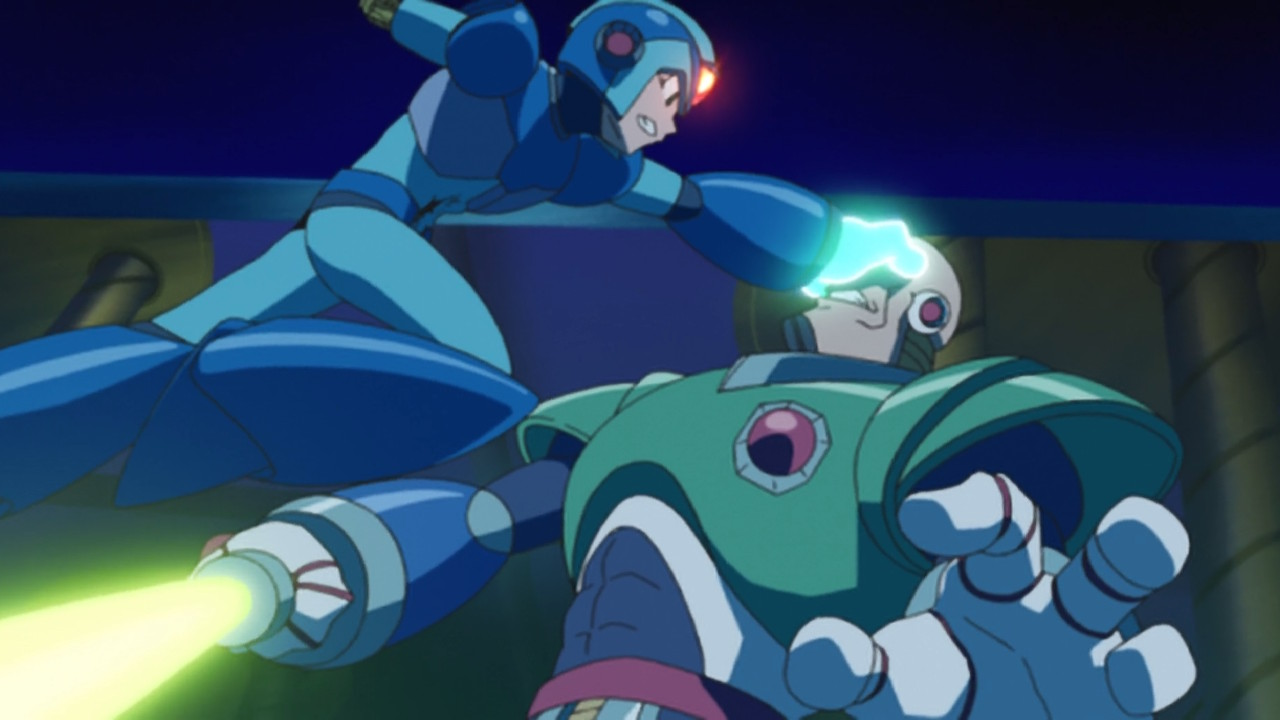
\includegraphics[width=.5\linewidth]{figures/X1/Sigma_scar.jpg}
	\caption{X burning Sigma's scars in.}
\end{figure}

After the rebellion's beginning, the few hunters remained loyal to their original purpose, X and Zero included, starting a period of wars which in future will be labeled as ``\emph{Maverick wars}''. 

From now on X's story follows the game's plot. During the event of the first game (and its remake) Zero is appointed as leader of the Maverick Hunters, being the highest in rank still on the right side, and leads other hunters, X included, in fighting. Zero then asks  X to take care of Sigma's subordinate both because their actions are causing trouble to humans and other reploids, but most importantly to allow X to grow up and become stronger, as Sigma is still too powerful for him. Once X disposes of the eight mavericks, Zero contacts him to ask help to infiltrate Sigma's fortress, which he managed to locate in the meanwhile. Once inside the two first challenge Vile, which results in his death but in Zero's death too. Finally X faces Sigma and defeats him, halting his plans of human extinction. After escaping Sigma's collapsing fortress, X returns to the Maverick Hunter headquarters, where he becomes the new leader in charge, under Dr.~Cain's direction.

Despite Sigma's defeat, however, Maverick attacks against humanity do not stop. This lead to more fights between mavericks and Mavericks Hunters for six more months, which results in heavy losses for both parts, reducing the number of effective Hunters to a quarter of its original number and also in the loss. Despite that, however, mavericks' numbers do not suffer the same loss, rising instead. This is caused by special factories which mavericks had previously altered to implant maverick chips into new reploids. After some searching Dr.~Cain manages to find the culprit factory, and X and the Maverick Hunters are dispatched to destroy it. Once arrived, X destroys the factory alongside the army of giant mechaniloid CF-0 which was produced. With this action X and the Hunters deal a heavy blow to mavericks forces, forcing the new leaders, the X-Hunters, to change their plans for the future and release their highest-ranked mavericks in order to buy them more time to complete their schemes. This plan too reveals to be a failure, since X manages to defeat his opponents much faster than expected, forcing the X-Hunters themselves to come out and face X, using the Zero's part they have repaired to lure X into fighting them. Despite this distraction, X manages to defeat all remaining high-ranked mavericks and proceeds to attack the X-Hunters fortress. 

At this point the story branches into two paths, both of which can be considered canonical. On one route X defeats all the X-Hunters and recovers all Zero's parts. Dr.~Cain then locates X-Hunters' secret base and proceeds to repair  Zero while X begins to attack the fortress. There X destroys all the three X-Hunters and discovers that Sigma is still alive, and waiting for him at the Central Computer. Once arrived, Sigma greets X and presents him a black clone of Zero, created by Serges, which he intends to use to destroy X. However the real Zero appears, destroys his clone and forces Sigma to retreat. Zero then opens a path for X to chase Sigma, and heads to destroy the main computer. Finally X faces Sigma, who in the fight reveals his true form as a Virus capable of manifesting into the real world, and defeats him again.

In the alternate route X fails to recover all Zero's parts. Here the X-Hunters attack Maverick Hunters HQ and steal all Zero's parts, control circuit included, and use them to revive Zero. From this point the narration follows the story described earlier except for the final part, where Sigma presents himself alongside the real Zero, now under Sigma's control. X and Zero fight, but the former manages to win, bringing Zero back to his senses. The plot then converges again into the same ending.



